\documentclass[12pt,a4paper,openany]{article}
\usepackage{lmodern}
\usepackage[table]{xcolor}
\usepackage{xcolor}
\definecolor{vert1}{rgb}{0.0,0.3.9,0.0}
\definecolor{bleu}{rgb}{0,0,0.5}
\definecolor{bleu3}{rgb}{1,0.2,0.2}
\definecolor{grisgris}{gray}{0.4}
\definecolor{rougeUPS}{rgb}{0.6, 0.3, 0.3}

\fboxsep =0pt \parindent =0pt\parskip =12pt



\usepackage[utf8]{inputenc} \usepackage[T1]{fontenc}
\usepackage[francais]{babel}
\usepackage[top=1.7cm, bottom=1.7cm, left=1.7cm, right=1.7cm]{geometry}
\usepackage{verbatim}
\usepackage[urlbordercolor={1 1 1}, linkbordercolor={1 1 1}, linkcolor=vert1, urlcolor=bleu, colorlinks=true]{hyperref}
\usepackage{tikz} %Vectoriel
\usepackage{listings}
\usepackage{fancyhdr}
\usepackage{multido}
\usepackage{float}
\usepackage{amssymb}

\newcommand{\titre}{Dossier de conception préliminaire}

\newcommand{\pole}{}
\newcommand{\sigle}{}

\newcommand{\semestre}{4}

\definecolor{gris1}{gray}{0.40}
\definecolor{gris2}{gray}{0.55}
\definecolor{gris3}{gray}{0.65}
\definecolor{gris4}{gray}{0.50}
\definecolor{vert}{rgb}{0,0.4,0}
\definecolor{violet}{rgb}{0.65, 0.2, 0.65}
\definecolor{bleu1}{rgb}{0,0,0.8}
\definecolor{bleu2}{rgb}{0,0.2,0.6}
\definecolor{bleu3}{rgb}{0,0.2,0.2}
\definecolor{rouge}{HTML}{F93928}


\lstdefinelanguage{algo}{%
   morekeywords={%
    %%% couleur 1
		importer, programme, glossaire, fonction, procedure, constante, type, 
	%%% IMPORT & Co.
		si, sinon, alors, fin, tantque, debut, faire, lorsque, fin lorsque, 
		declenche, declencher, enregistrement, tableau, retourne, retourner, =, pour, a,
		/=, <, >, traite,exception, 
	%%% types 
		Entier, Reel, Booleen, Caractere, Réél, Booléen, Caractère,
	%%% types 
		entree, maj, sortie,entrée,
	%%% types 
		et, ou, non,
	},
  sensitive=true,
  morecomment=[l]{--},
  morestring=[b]',
}

\lstset{language=algo,
    %%% BOUCLE, TEST & Co.
      emph={importer, programme, glossaire, fonction, procedure, constante, type},
      emphstyle=\color{bleu2},
    %%% IMPORT & Co.  
	emph={[2]
		si, sinon, alors, fin , tantque, debut, faire, lorsque, fin lorsque, 
		declencher, retourner, et, ou, non,enregistrement, retourner, retourne, 
		tableau, /=, <, =, >, traite,exception, pour, a
	},
      emphstyle=[2]\color{bleu1},
    %%% FONCTIONS NUMERIQUES
      emph={[3]Entier, Reel, Booleen, Caractere, Booléen, Réél, Caractère},
      emphstyle=[3]\color{gris1},
    %%% FONCTIONS NUMERIQUES
      emph={[4]entree, maj, sortie, entrée},	
      emphstyle=[4]\color{gris1},
}
\lstdefinelanguage{wl}{%
   morekeywords={%
    %%% couleur 1
		importer, programme, glossaire, fonction, procedure, constante, type, 
	%%% IMPORT & Co.
		si, sinon, alors, fin, TANTQUE, tantque, FIN, PROCEDURE, debut, faire, lorsque, 
		fin lorsque, declenche, declencher, enregistrement, tableau, retourne, retourner, =, 
		/=, <, >, traite,exception, 
	%%% types 
		Entier, Reel, Booleen, Caractere, Réél, Booléen, Caractère,
	%%% types 
		entree, maj, sortie,entrée,
	%%% types 
		et, ou, non,
	},
  sensitive=true,
  morecomment=[l]{//},
  morestring=[b]',
}

\lstset{language=wl,
    %%% BOUCLE, TEST & Co.
      emph={importer, programme, glossaire, fonction, procedure, constante, type},
      emphstyle=\color{bleu2},
    %%% IMPORT & Co.  
	emph={[2]
		si, sinon, alors, fin , tantque, debut, faire, lorsque, fin lorsque, 
		declencher, retourner, et, ou, non,enregistrement, retourner, retourne, 
		tableau, /=, <, =, >, traite,exception
	},
      emphstyle=[2]\color{bleu1},
    %%% FONCTIONS NUMERIQUES
      emph={[3]Entier, Reel, Booleen, Caractere, Booléen, Réél, Caractère},
      emphstyle=[3]\color{gris1},
    %%% FONCTIONS NUMERIQUES
      emph={[4]entree, maj, sortie, entrée},	
      emphstyle=[4]\color{gris1},
}
\lstdefinelanguage{css}{%
   morekeywords={%
    %%% couleur 1
		background, image, repeat, position, index, color, border, font, 
		size, url, family, style, variant, weight, letter, spacing, line, 
		height, text, decoration, align, indent, transform, shadow, 
		background, image, repeat, position, index, color, border, font, 
		size, url, family, style, variant, weight, letter, spacing, line, 
		height, text, decoration, align, indent, transform, shadow, 
		vertical, align, white, space, word, spacing,attachment, width, 
		max, min, margin, padding, clip, direction, display, overflow,
		visibility, clear, float, top, right, bottom, left, list, type, 
		collapse, side, empty, cells, table, layout, cursor, marks, page, break,
		before, after, inside, orphans, windows, azimuth, after, before, cue, 
		elevation, pause, play, during, pitch, range, richness, spek, header, 
		numeral, punctuation, rate, stress, voice, volume,
	%%% types 
		left, right, bottom, top, none, center, solid, black, blue, red, green,
	},
  sensitive=true,
  sensitive=true,
  morecomment=[s]{/*}{*/},
  morestring=[b]',
}
\lstset{language=css,
    %%% BOUCLE, TEST & Co.
      emph={
		background, image, repeat, position, index, color, border, font, 
		size, url, family, style, variant, weight, letter, spacing, line, 
		height, text, decoration, align, indent, transform, shadow, 
		background, image, repeat, position, index, color, border, font, 
		size, url, family, style, variant, weight, letter, spacing, line, 
		height, text, decoration, align, indent, transform, shadow, 
		vertical, align, white, space, word, spacing,attachment, width, 
		max, min, margin, padding, clip, direction, display, overflow,
		visibility, clear, float, top, right, bottom, left, list, type, 
		collapse, side, empty, cells, table, layout, cursor, marks, page, break,
		before, after, inside, orphans, windows, azimuth, after, before, cue, 
		elevation, pause, play, during, pitch, range, richness, spek, header, 
		numeral, punctuation, rate, stress, voice, volume,
	  },
      emphstyle=\color{bleu2},
    %%% FONCTIONS NUMERIQUES
      emph={[3]
		left, right, bottom, top,none, solid, black, blue, green,
		  },
      emphstyle=[3]\color{bleu3},
    %%% FONCTIONS NUMERIQUES
}

\lstset{language=SQL,
    %%% BOUCLE, TEST & Co.
      emph={INSERT, UPDATE, DELETE, WHERE, SET, GROUP, BY, ORDER},
      emphstyle=\color{bleu2},
    %%% IMPORT & Co.  
	emph={[2]
		if, end, begin, then, for, each, else, after, of, on, to
	},
      emphstyle=[2]\color{bleu1},
    %%% FONCTIONS NUMERIQUES
      emph={[3]Entier, Reel, Booleen, Caractere, Booléen, Réél, Caractère},
      emphstyle=[3]\color{gris1},
    %%% FONCTIONS NUMERIQUES
      emph={[4]entree, maj, sortie, entrée},	
      emphstyle=[4]\color{gris1},
}
\lstdefinelanguage{ARM}{%
   morekeywords={%
   ADD, SUB, MOV, MUL, RSB,CMP, BLS, BLE, B,BHI,
   BGE, RSBLT, BGT, BEQ, BNE,BLT
	},
  sensitive=true,
  morecomment=[l]{@},
  morestring=[b]',
}

\lstset{ % general style for listings 
   numbers=left 
   , literate={é}{{\'e}}1 {è}{{\`e}}1 {à}{{\`a}}1 {ê}{{\^e}}1 {É}{{\'E}}1 {ô}{{\^o}}1 {€}{{\euro}}1{°}{{$^{\circ}$}}1 {ç}{ {c}}1
	, extendedchars=\true
   , tabsize=2 
   , frame=l
   , framerule=1.1pt
   , linewidth=520px
   , breaklines=true 
   , basicstyle=\footnotesize\ttfamily 
   , numberstyle=\tiny\ttfamily 
   , framexleftmargin=0mm 
   , xleftmargin=0mm 
   , captionpos=b 
	, keywordstyle=\color{bleu2}
	, commentstyle=\color{vert}
	, stringstyle=\color{rouge}
	, showstringspaces=false
	, extendedchars=true
	, mathescape=true
} 
%	\lstlistoflistings
%	\addcontentsline{toc}{part}{List of code examples}

\date{\today}

\makeindex
\lfoot{Université Toulouse III -- Paul Sabatier}
\rfoot{}
%\rfoot{}
\cfoot{}
\makeglossary
\makeatletter
\def\clap#1{\hbox to 0pt{\hss #1\hss}}%
\def\ligne#1{%
\hbox to \hsize{%
\vbox{\centering #1}}}%
\def\haut#1#2#3{%
\hbox to \hsize{%
\rlap{\vtop{\raggedright #1}}%
\hss
\clap{\vtop{\centering #2}}%
\hss
\llap{\vtop{\raggedleft #3}}}}%
\def\bas#1#2#3{%
\hbox to \hsize{%
\rlap{\vbox{\raggedright #1}}%
\hss \clap{\vbox{\centering #2}}%
\hss
\llap{\vbox{\raggedleft #3}}}}%
\def\maketitle{%
\thispagestyle{empty}\vbox to \vsize{%
\haut{}{\@blurb}{}

\vfill
\vspace{1cm}
\begin{flushleft}
\usefont{OT1}{ptm}{m}{n}
\huge \@title
\end{flushleft}
\par
\hrule height 4pt
\par
\begin{flushright}
\usefont{OT1}{phv}{m}{n}
\Large \@author
\par
\end{flushright}
\vspace{1cm}
\vfill
\vfill
\bas{}{\@location, le \@date}{}
}%
\cleardoublepage
}
\def\date#1{\def\@date{#1}}
\def\author#1{\def\@author{#1}}
\def\title#1{\def\@title{#1}}
\def\location#1{\def\@location{#1}}
\def\blurb#1{\def\@blurb{#1}}
\date{\today}
\author{}
\title{}
\location{Amiens}\blurb{}
\makeatother
\title{\titre}
\author{Projet de Boggle}

\location{Toulouse}
\blurb{%
Université Toulouse III -- Paul sabatier\\
L2 Informatique\\
Projet tuteuré\\
\vspace{30px}
\begin{flushleft}Antoine de \bsc{Roquemaurel}\\ Fabrice
	\bsc{Valleix}\\ Groupe 2.2\end{flushleft}
}%



%\title{Cours \\ \titre}
%\date{\today\\ Semestre \semestre}

%\lhead{Cours: \titre}
%\chead{}
%\rhead{\thepage}

%\lfoot{Université Paul Sabatier Toulouse III}
%\cfoot{\thepage}
%\rfoot{\sigle\semestre}

\pagestyle{fancy}
%\renewcommand{\chaptermark}[1]{\markboth{\bsc{\chaptername~\thechapter{} :} #1}{}}
\renewcommand{\sectionmark}[1]{\markright{\thesection{ #1}}}
\renewcommand{\headrulewidth}{0.3pt}
\renewcommand{\footrulewidth}{0.3pt}

\fancyhf{}
\fancyhead[LO]{Antoine de \bsc{Roquemaurel} -- Fabrice \bsc{Valleix}}
\fancyhead[RO]{\rightmark}
\fancyfoot[CO]{--~\thepage~--}
\fancyfoot[LO]{Dossier de spécifications}
\fancyfoot[RO]{Projet de Boggle}
\fancyfoot[RE]{Antoine de \bsc{Roquemaurel} -- Fabrice \bsc{Valleix}}

%% Cas des premières pages de chapitre
\fancypagestyle{plain}{%
	\fancyhf{}%
	\fancyfoot[L]{\titre{}}
	\fancyfoot[R]{--~\thepage~--}
	\renewcommand{\headrulewidth}{0pt}
	\renewcommand{\footrulewidth}{0.3pt}
}
\makeatletter
\renewcommand*{\lstlistlistingname}{Liste des codes sources}
\renewcommand{\listfigurename}{Liste des figures}
\renewcommand\listoffigures{%
    \subsection{\listfigurename}%
      \@mkboth{\MakeUppercase\listfigurename}%
              {\MakeUppercase\listfigurename}%
       \@starttoc{lof}%
    }
    \renewcommand\listoftables{%
    \subsection{\listtablename}%
    \@mkboth{\MakeUppercase{\listtablename}}%
            {\MakeUppercase{\listtablename}}%
    \@starttoc{lot}
    }

    \renewcommand\lstlistoflistings{%
    \begingroup
    \subsection{\lstlistlistingname}%
    \parskip\z@\parindent\z@\parfillskip \z@ \@plus 1fil%
    \@starttoc{lol}%
    \endgroup
    }
	\makeatother

\definecolor{exemple}{HTML}{dde5ed}
\definecolor{remarque}{HTML}{dde5ed}
\newcommand{\exemple}[1]{
	\begin{center}
	\medskip
	\colorbox{exemple}{
	\begin{minipage}{0.8\textwidth}\vspace{10px}\textbf{Ex }\medskip#1 \medskip\end{minipage}
	}
	\medskip
	\end{center}
}
\newcommand{\remarque}[1]{
	\begin{center}
	\medskip
	\colorbox{remarque}{
		\begin{minipage}{0.8\textwidth}\medskip\includegraphics[height=10px]{/home/aroquemaurel/cours/includesLaTeX/images/remarque.png} #1 \medskip\end{minipage}
	}
	\medskip
	\end{center}
}

\newcommand{\attention}[1]{
	\begin{center}
	\medskip
	\colorbox{remarque}{
		\begin{minipage}{0.8\textwidth}\medskip\includegraphics[height=10px]{/home/aroquemaurel/cours/includesLaTeX/images/attention.png} #1 \medskip\end{minipage}
	}
	\medskip
	\end{center}
}

\DeclareTextFontCommand{\policeGlossaire}{\fontfamily{lmss}\selectfont}
\DeclareTextFontCommand{\policePackage}{\fontfamily{phv}\selectfont}
\DeclareTextFontCommand{\policeTitre}{\fontfamily{ptm}\selectfont}
\newcommand{\policeCode}[1]{\texttt{#1}}

\newcommand{\sectionfont}{%
	\fontencoding{\encodingdefault}%
	\fontfamily{pag}%
	\fontseries{bc}%
	\fontshape{n}%
	\selectfont
}

% numéro du chapitre
\DeclareFixedFont{\chapnumfont}{T1}{phv}{b}{n}{80pt}
% pour le mot « Chapitre »
\DeclareFixedFont{\chapchapfont}{T1}{phv}{b}{n}{16pt}
% pour le titre
\DeclareFixedFont{\chaptitfont}{T1}{phv}{b}{n}{24.88pt}


\makeatletter
\def\thickhrulefill{\leavevmode \leaders \hrule height 1ex \hfill \kern \z@}

\newlength{\sectiontitleindent}
\newlength{\subsectiontitleindent}
\newlength{\subsubsectiontitleindent}
\setlength{\sectiontitleindent}{-1cm}
\setlength{\subsectiontitleindent}{-.5cm}
\setlength{\subsubsectiontitleindent}{-.25cm}

\renewcommand{\section}{%
	\@startsection%
	{section}%
	{1}%
	{\sectiontitleindent}%
	{-3.5ex plus -1ex minus -.2ex}%
	{2.3ex plus.2ex}%
	{\sectionfont\Large}
}
\renewcommand{\subsection}{%
	\@startsection%
	{subsection}%
	{2}%
	{\subsectiontitleindent}%
	{-3.5ex plus -1ex minus -.2ex}%
	{2.3ex plus.2ex}%
	{\sectionfont\large}
}

\renewcommand{\subsubsection}{%
	\@startsection%
	{subsubsection}%
	{3}%
	{\subsubsectiontitleindent}%
	{-3.5ex plus -1ex minus -.2ex}%
	{2.3ex plus.2ex}%
	{\sectionfont\normalsize}
}

\makeatother

\newcommand{\lien}[1]{
 $\vartriangleright$ \url{#1}
 }

\newcommand{\pfp}{\texttt{pfp}}

\newcommand{\ifp}{\texttt{if}}
\newcommand{\elsep}{\texttt{else}}

\makeatother
\includeonly {
}
\begin{document}
	\setcounter{tocdepth}{2}
	\setcounter{secnumdepth}{3}
	\maketitle
	\tableofcontents
	\newpage
	\section{But du document}
	C'est une description de haut niveau du produit, c'est-à-dire l'architecture générale du système, en termes de << modules >>, de sous modules et de leurs
	interactions. De plus, chaque module doit être décrit (définition des interfaces et des fonctionnalités générales). Ce document doit en premier lieu asseoir
	la confiance en la finalité et la faisabilité du produit, et, en second lieu, servir de base pour l'estimation des tâches à effectuer et du calendrier de
	leur réalisation.

	Le << Dossier de Conception Préliminaire >> doit également mettre en évidence le plan de tests, en termes de besoins de l'utilisateur, et montrer que l'on peut
	y satisfaire grâce à l'architecture proposée.
	\section{Diagramme de décomposition en modules}\label{diagModules}
	La description détaillée des différents modules est disponible section \ref{listeModules}. 
	\remarque{Afin de ne pas surcharger le schéma, le module \texttt{Utile} n'a
	pas été représenté ici, en effet tous les modules du projet sont susceptibles d'en avoir besoin, de plus ce module ne contient pas de fonctions spécifiques
	au projet mais des fonctions utiles travaillant sur des types de bases.}
	\begin{figure}[H]
		\centering
		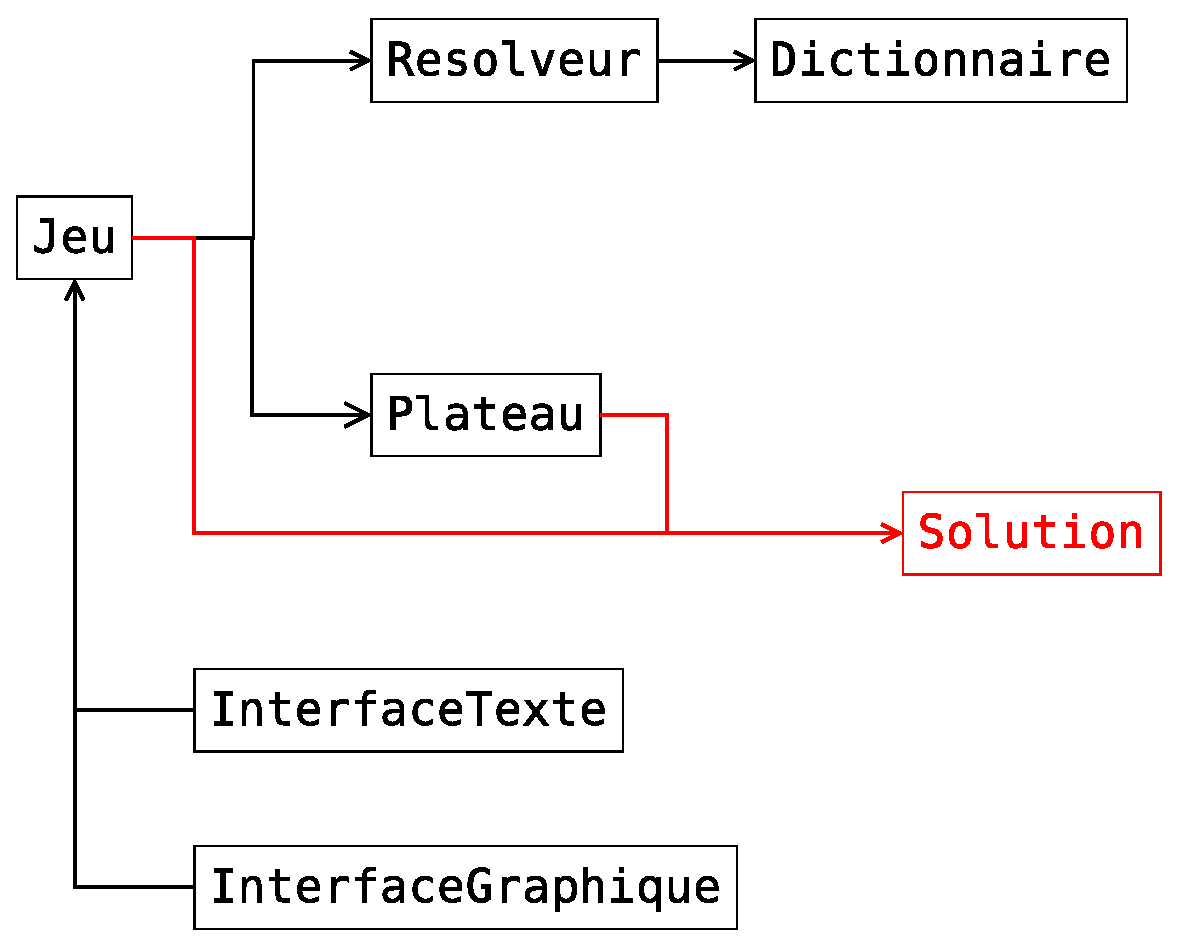
\includegraphics[width=8cm]{diagrammeModules.eps}
		\caption{Diagramme de décomposition en modules}
	\end{figure}
	\section{Description des différents modules}\label{listeModules}
	Un diagramme représentant l'interaction entre les différents modules est disponible section \ref{diagModules}.
	\subsection{Module \texttt{Utile}}\label{utile}
		\begin{table}[H]
		\rowcolors{1}{grisgris}{}
			\centering
		\begin{tabular}{p{5cm} p{12cm}}
			\textbf{Rôle} & Toutes les fonctions de bases utiles au projet, ces fonctions tra\-vaillent sur des types de bases et ne sont pas spécifiques au
			projet, mais ce module permet de mieux organiser le code. \\
			\textbf{Type de données} & Contient uniquement des traitements\\ 
			\textbf{Dépendances} & Aucune\\ 
			\textbf{Fonctionnalités fournies} & La liste sera complété au fur et a mesure du projet en
			fonction des besoin nécessaires, en voici déjà quelques une: supprimer les accents d'une chaine de caractère, mettre une chaine de caractère en
			majuscule, n'afficher un message qu'en cas de mode debug, trouver la première chaine de caractère présente dans un tableau, retourner un booléen en
			fonction d'une certaine probabilité, etc\ldots 
		\end{tabular}
		\caption{Module \texttt{Utile}}
	\end{table}
	\subsection{Module \texttt{Plateau}}\label{plateau}
		\begin{table}[H]
		\rowcolors{1}{grisgris}{}
			\centering
		\begin{tabular}{p{5cm} p{12cm}}
			\textbf{Rôle} & Gérer la grille de Boggle\\
			\textbf{Type de données} & Tableau à deux dimensions de \texttt{char} \\
			\textbf{Dépendances} & \texttt{Utile}(\ref{utile})\\
			\textbf{Fonctionnalités fournies} & Générer la grille, Retourner la lettre concernant une case donnée\\
		\end{tabular}
		\caption{Module \texttt{Plateau}}
	\end{table}
	\subsection{Module \texttt{Dictionnaire}}\label{dictionnaire}
		\begin{table}[H]
		\rowcolors{1}{grisgris}{}
			\centering
		\begin{tabular}{p{5cm} p{12cm}}
			\textbf{Rôle} & Gérer le dictionnaire du Boggle\\
			\textbf{Type de données} & Fichier \texttt{FILE*} pointant sur le dictionnaire\\
			\textbf{Dépendances} & \texttt{Utile}(\ref{utile})\\
			\textbf{Fonctionnalités fournies} & Initialiser le dictionnaire, parcourir le dictionnaire, dire si un mot est présent dans le dictionnaire ou non. 
		\end{tabular}
		\caption{Module \texttt{Dictionnaire}}
	\end{table}
	\subsection{Module \texttt{Resolveur}}\label{resolveur}
		\begin{table}[H]
		\rowcolors{1}{grisgris}{}
			\centering
		\begin{tabular}{p{5cm} p{12cm}}
			\textbf{Rôle} & Résoudre une grille de Boggle\\
			\textbf{Type de données} & Structure contenant la grille de Boggle, le dictionnaire et un tableau de \texttt{char*} avec tous les mots possibles\\
			\textbf{Dépendances} & \texttt{Dictionnaire}(\ref{dictionnaire}), \texttt{Plateau}(\ref{plateau}), \texttt{Utile}(\ref{utile})\\
			\textbf{Fonctionnalités fournies} & Résoudre la grille, signaler si un mot est présent dans la grille, retourner la liste des mots de la grille
			commençant par une lettre. 
		\end{tabular}
		\caption{Module \texttt{Resolveur}}
	\end{table}
	\subsection{Module \texttt{Jeu}}\label{jeu}
		\begin{table}[H]
		\rowcolors{1}{grisgris}{}
			\centering
		\begin{tabular}{p{5cm} p{12cm}}
			\textbf{Rôle} & Jouer au Boggle \\ 
			\textbf{Type de données} & Structure contenant le Plateau et le Résolveur\\ 
			\textbf{Dépendances} & \texttt{Plateau}(\ref{plateau}), \texttt{Resolveur}(\ref{resolveur}), \texttt{Utile}(\ref{utile})\\
			\textbf{Fonctionnalités fournies} & Proposer une lettre, Lancer le compte à rebours, Signaler si un mot proposé est correct, retourner le nombre de
			point obtenus, signaler si le joueur à gagner le jeu ou non
		\end{tabular}
		\caption{Module \texttt{Jeu}}
	\end{table}
		\subsection{Module \texttt{InterfaceTexte}}
		\begin{table}[H]
		\rowcolors{1}{grisgris}{}
			\centering
		\begin{tabular}{p{5cm} p{12cm}}
			\textbf{Rôle} & Afficher et permettre de jouer au Boggle en mode texte\\ 
			\textbf{Type de données} & \texttt{Jeu}\\ 
			\textbf{Dépendances} & \texttt{Jeu}(\ref{jeu}), \texttt{Utile}(\ref{utile})\\ 
			\textbf{Fonctionnalités fournies} & Toutes les fonctions d'affichage et de saisie
		\end{tabular}
		\caption{Module \texttt{InterfaceTexte}}
	\end{table}
		\subsection{Module \texttt{InterfaceGraphique}}
		\begin{table}[H]
		\rowcolors{1}{grisgris}{}
			\centering
		\begin{tabular}{p{5cm} p{12cm}}
			\textbf{Rôle} & Afficher et permettre de jouer au Boggle en mode semi graphique\\ 
			\textbf{Type de données} & \texttt{Jeu}(\ref{jeu})\\ 
			\textbf{Dépendances} & \texttt{Jeu}, bibliothèque externe \texttt{ncurses}, \texttt{Utile}\\ 
			\textbf{Fonctionnalités fournies} & Toutes les fonctions d'affichage et de saisie
		\end{tabular}
		\caption{Module \texttt{InterfaceGraphique}}
	\end{table}
	\section{Répartition des tâches entre chaque membre}
	Un module sera toujours affecté à un membre du groupe, celui-ci sera en charge de vérifier que le module avance dans le temps impartis, et de s'occuper de
	l'intégration. Chacune des tâches seront affecté à un membre du groupe qui devra implémenter la tâche dans les délais prévus.

	Le module \texttt{Utile} ne possède personne qui lui est assigné, en effet ce module se remplira en fonction de l'avancement des autres modules, et sera donc
	développé par les deux membres du binôme tout au long du projet.
	\begin{figure}[H]
		\centering
		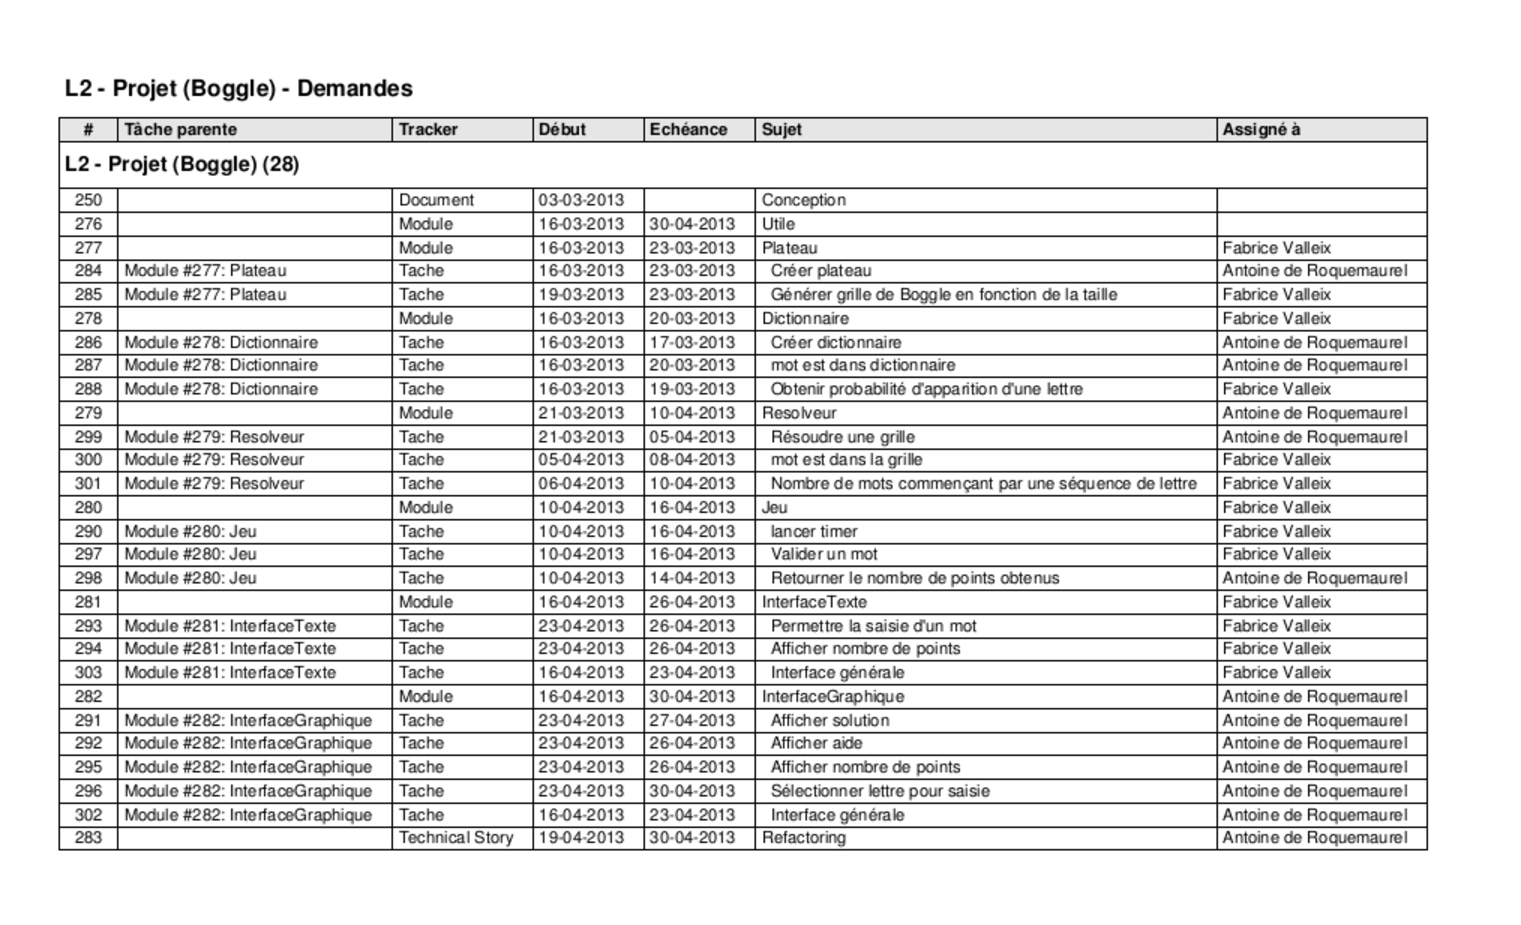
\includegraphics[angle=-90,width=15.2cm]{taches.pdf}
		\caption{Liste des tâches et leur répartition}
	\end{figure}
	\section{Calendrier de réalisation des tâches}
	\begin{figure}[H]
		\centering
		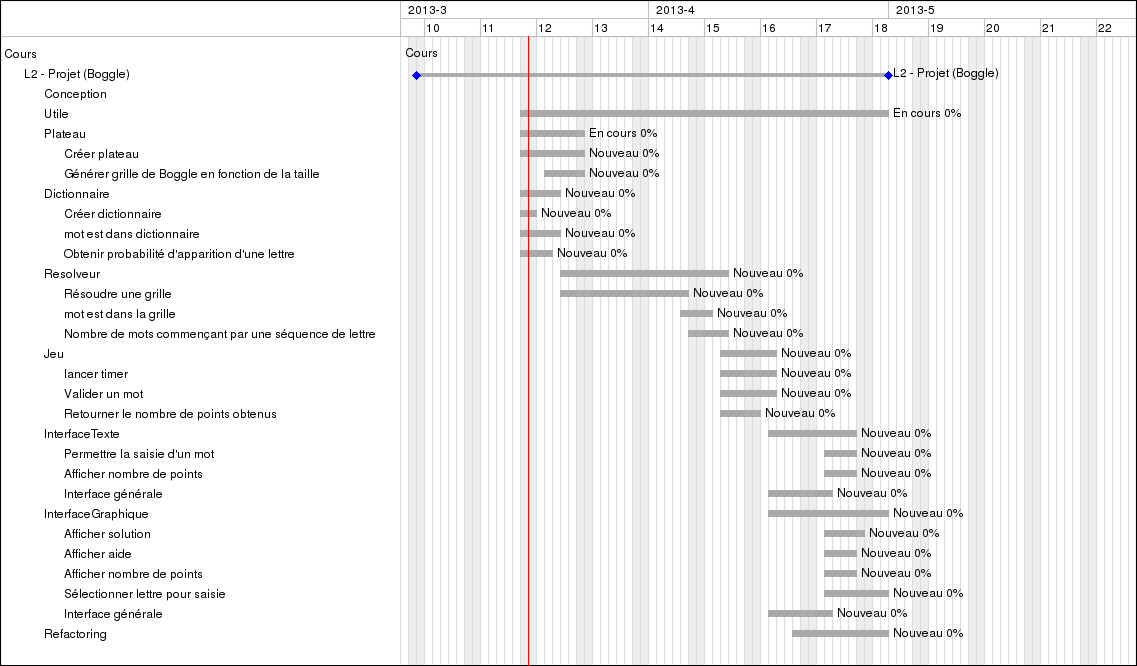
\includegraphics[angle=-90,width=14.2cm]{gantt.png}
		\caption{Diagramme de Gantt}
	\end{figure}
	\section{Plan de tests}
	Chaque fonction de chaque module sera testée à l'aide de tests unitaire, s'appuyant sur la bibliothèque \texttt{cunit}. Chacun des tests unitaire au pour but
	de tester un et un seul cas, mais l'ensemble des tests unitaires d'un module devront avoir passer en revue tous les cas possibles d'appel d'une fonction :
	Que ce soit un cas nominal, ou un cas d'erreur, ainsi chacune des lignes de code auront été testé, si ce n'est pas possible, du code mort aura été détecté. 

	Une fois que chaque fonction aura passé les tests unitaires, nous allons tester les modules séparément afin de vérifier que toutes les fonctions fonctionnent
	bien entre elle, ces tests seront différents en fonctions des modules.

	\subsection{Plateau}
		Un test fonctionnel aura lieu afin de tester le module, pour cela, nous appellerons la fonction de génération de grille et vérifierons qu'elle a bien
		généré une grille en fonction des tailles que nous lui donnons. Un jeu de grille sera généré, afin de vérifier que les lettres présentes dans la grilles
		le sont en fonction de leur utilisation dans la langue Française, un facteur de probabilité entrant en compte, il n'est pas possible d'attendre une
		réponse exacte.

		Ce test s'effectuera tout d'abord dans son fonctionnement nominal, pour toutes les tailles que l'utilisateur est susceptible de rentrer (de 2 à 15, cette
		taille étant fixée dans les spécifications), ensuite un test s'effectuera sur des valeurs alternatives : nombre négatif, flottants, supérieur à 15
		etc\ldots et nous vérifierons que les erreurs sont bien gérés.
	\subsection{Dictionnaire}
		Afin de tester le dictionnaire, il faudra vérifier que la fonction permettant de savoir si un mot est présent dans le
		dictionnaire est correcte. Afin de tester cette fonction nous aurons un jeu d'essai comportant des mots présents, ou non dans la dictionnaire, au début
		du dictionnaire, à la fin, ou au milieu, des mots de longueur variable allant de 3 caractères, jusqu'à des mots de 20 caractères  
		et vérifierons que les retour de fonctions sont bien ceux attendus.

	\subsection{Résolveur}
		Pour tester le Résolveur, nous essayerons avec des grilles prédéfinis de tailles variables, et vérifierons que le résolveur retourne bien tous les
		mots présent dans ces grilles, ceci sans erreurs. Le résolveur dépendant du dictionnaire, nous devons avoir testé préalablement le dictionnaire afin de
		pouvoir tester ce module.

		Afin de vérifier tous les cas possibles, nous utiliserons le plus de grilles possible, tout d'abord des grilles classiques de taille $4\times4$, 
		avec le plus de mots possibles présent dans la grille. Ensuite nous testerons le résolveur sur des grilles de taille $15\times 15$ afin de 
		vérifier qu'il n'est pas trop lent par rapport à ce que nous avions énoncé dans les spécifications. Également, nous lui
		ferons passer une grille ou aucun mot n'est possible dans la grille et une grille de taille $2\times 2$ afin de vérifier que dans ces cas extrêmes, le module fonctionne correctement.

	\subsection{Jeu}
	Afin de tester ce module, une interface est indispensable, ainsi nous nous en tiendrons aux tests unitaires, afin de vérifier que toutes les fonctions du
	module fonctionnent, ensuite ce module sera testé via l'intermédiaire de l'interface en mode texte.

	\subsection{\texttt{InterfaceGraphique} et \texttt{InterfaceTexte}}
	Ces deux modules sont les interfaces du jeu, il est difficile de faire des tests automatisé pour les interfaces, de plus ces deux modules sont intimement
	liés au contrôleur, \texttt{Jeu}, ainsi nous ne pourrons pas tester les interfaces séparément des autres modules, ces deux interfaces seront donc testé à
	l'aide d'un test fonctionnel lors d'une partie de Boggle. Ce test s'effectuera avec une grille prédéfinie.

	\subsection{Globalité}
	Une fois tous les tests effectué, nous testerons l'application complète, génération de la grille inclue, en spécifiant des tailles de grilles différentes,
	allant de 2 à 15.

	% Test fonctionnel de l'application en mode text et en mode semi-graphique avec une grille non générée
	\newpage
	\appendix
	\section{Annexes}
	\listoffigures
	\listoftables
	
\end{document}

